 $Datalog^M$ supports cross-compilation, or pretty-printing, to Souffle. The pretty-printing implementation nicely highlights the power of JastAdd. The AST is kept in a Java class hierarchy with ASTNode as a common ancestor of all classes.
Aspects enable the addition of methods to a generated AST-class. An overview of the design for extensible pretty-printing is shown in in figure \ref{figure:pretty}. To enable re-use of existing pretty-printing functionality, the argument, \textit{PrettyPrinter}, recursively calls back into the corresponding printing method. The evaluation then proceeds by mutual recursion between \textit{pretty} and \textit{souffle}. In this way, a new pretty-printer can be added that alters or mixes the behavior of existing pretty-printers. The type-checking program is generated in the same way by declaring a \textit{TypePrettyPrinter} class.

% as well as for the type checking and inference program described in the previous section

\begin{figure}[!ht]
\begin{minted}{yaml}
void ASTNode.pretty(PrettyPrinter pr)  { ... }
void ASTNode.souffle(PrettyPrinter pr) { ... }
abstract class PrettyPrinter<T extends ASTNode> 
...
    abstract void pretty(T node);
...
class StandardPrettyPrinter extends PrettyPrinter 
...
    void pretty(T node) { node.pretty(this); }
...
class SoufflePrettyPrinter  extends PrettyPrinter 
... 
    void pretty(T node) { node.souffle(this); }
...
\end{minted}
\caption{The basis for pretty-printing and re-use through mutual recursion.}
\label{figure:pretty}
\end{figure}

\begin{figure*}[!ht]
	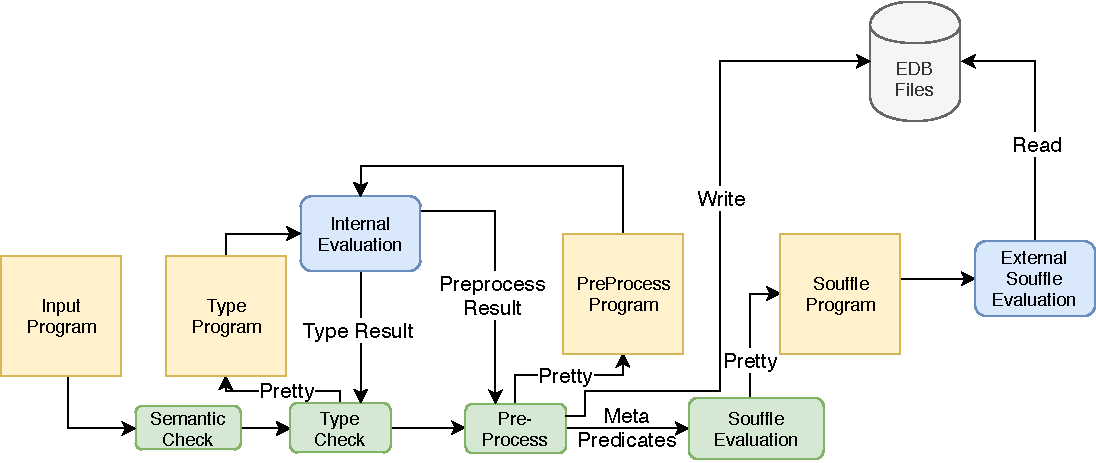
\includegraphics{img/souffleEval.pdf}
	\caption{Souffle Printing Pipeline. \textbf{Yellow}: A Datalog Program. \textbf{Blue}: An evaluation mechanism. \textbf{Green}: A compiler stage. }
	\label{figure:soufflePipeline}
\end{figure*}
\noindent
\subsection{Souffle Evaluation}
Souffle does not support meta-predicates and so naturally it does not recognize the meta-semantics introduced in the previous section. In particular the presence of meta-predicates that the interpreter provides to the Datalog program will fail if a straight forward pretty-printing is performed. The obvious solution then is to first evaluate the Datalog program up to the point that all such predicates are known in a pre-processing step. All the derived special predicates can then be provided to Souffle as additional facts by printing them in the pretty-printing step.